\chapter{Evaluation}
\label{ch:evaluation}

In this chapter, we will look at the results of the different models. 
We first evaluate which features are most important for the models using 
permutation feature importance, then we will look at the pinball scores from 
that are used in the competition. Finally, we will look at how the models performed 
considering another scoring function, the Energy score as well as the probabilistic calibration 
of the models using PIT histograms.

Before we look at the different evaluation metrics, 
we take a quick look at what the models predicted. 
Figure \ref{fig:predictions} shows the \(0.1, 0.5\) and \(0.9\)-percentile 
of the predicted distribution as well as the actual target data.
We can observe that the predictions for the Quantile Random Forests in Figure \ref{fig:predictions-qrf} are 
capped at the top values. 

\begin{figure}[h]%
    \centering
    \subfloat[\centering Quantile Random Forests]{{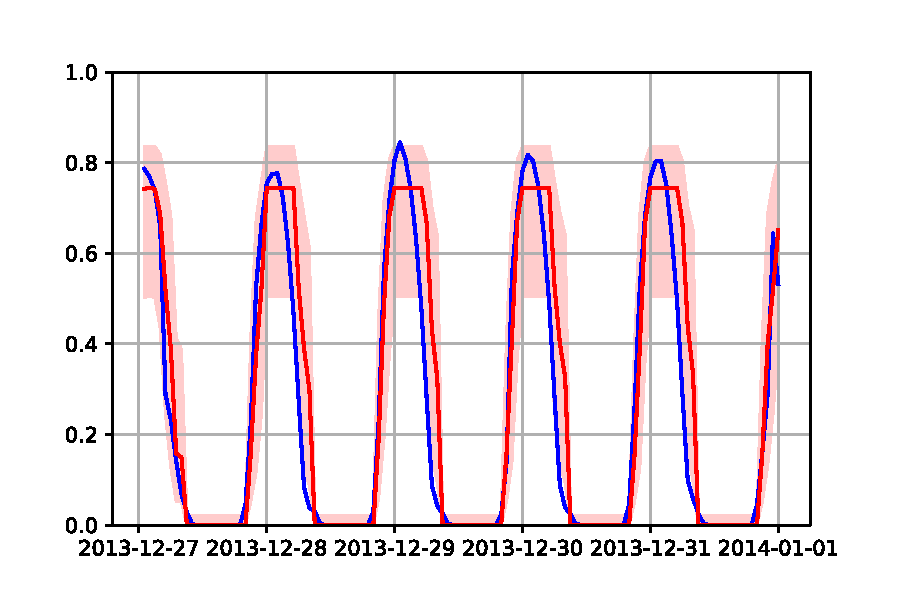
\includegraphics[width=0.3\textwidth]{plots/predictions/qrf_plot_9.pdf} \label{fig:predictions-qrf} }}
    \subfloat[\centering Nearest Neighbor Quantile Filters]{{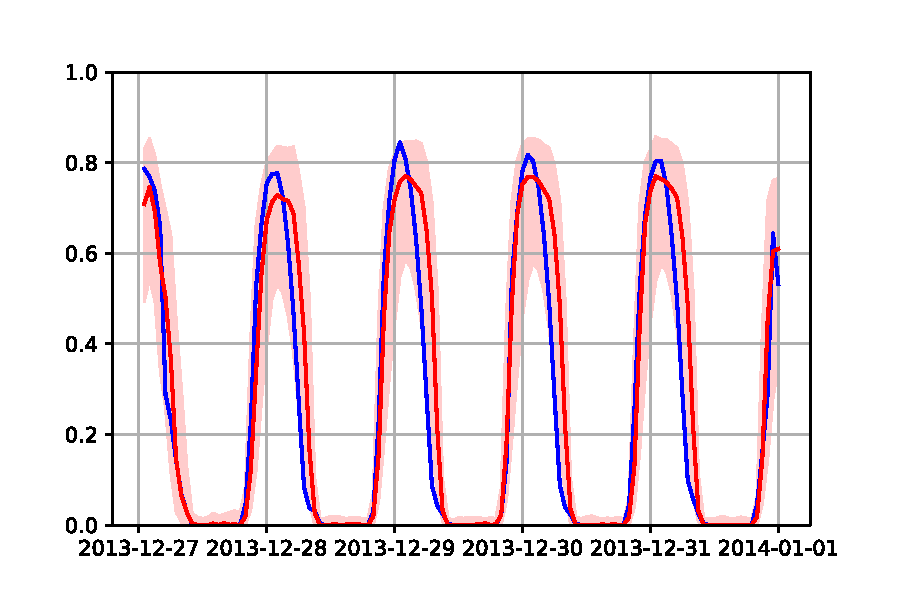
\includegraphics[width=0.3\textwidth]{plots/predictions/nnqf_plot_9.pdf} \label{fig:predictions-nnqf} }}
    \subfloat[\centering Spline Quantile Functions RNN]{{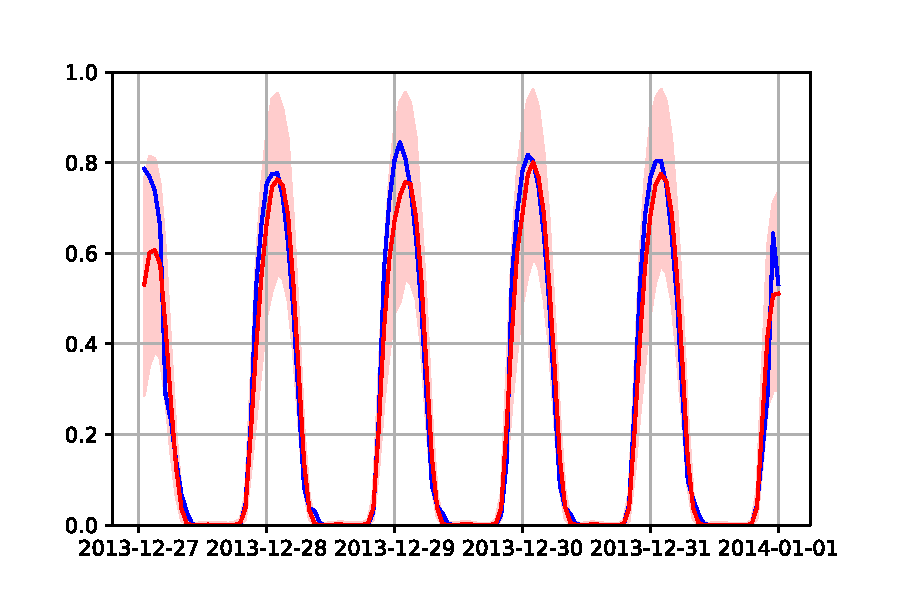
\includegraphics[width=0.3\textwidth]{plots/predictions/sqf_rnn_plot_9.pdf} \label{fig:predictions-sqf-rnn} }}
    \caption[Predictions]{Predictions of the forecasters. The \(0.1\) and \(0.9\) percentiles are shown in light red, the median in red and the actual data is the blue line.}%
    \label{fig:predictions}%
\end{figure}

\section{Feature importance}
\label{sec:feature-importance}

One way to determine the importance of a feature for a model is called 
permutation feature importance. Here, the model is trained like usual but for the prediction 
step, we don't use the normal test data, but a modified dataset where one feature is 
shuffled. Like that, the model cannot use the information of this feature properly 
and will most likely perform worse. The performance on the shuffled dataset is 
then divided by the performance on the regular test set. A value close to \(1\) 
indicates that the feature is not that important because the model doesn't perform 
much worse than before. The higher the quotient, the more important the feature is for the model.
Since our time series heavily depends of the time of day, it makes sense 
not to shuffle the whole feature but only the equivalence classes of each hour, 
i.e. the values at \(1\) AM are shuffled, the values at \(2\) AM are shuffled, etc.

Figure \ref{fig:feature-importance} 
shows the results of the permutation feature importance calculation.

\begin{figure}[h!]
    \section{Feature importance}
\label{sec:feature-importance}

One way to determine the importance of a feature for a model is called 
permutation feature importance. Here, the model is trained like usual but for the prediction 
step, we don't use the normal test data, but a modified dataset where one feature is 
shuffled. Like that, the model cannot use the information of this feature properly 
and will most likely perform worse. The performance on the shuffled dataset is 
then divided by the performance on the regular test set. A value close to \(1\) 
indicates that the feature is not that important because the model doesn't perform 
much worse than before. The higher the quotient, the more important the feature is for the model.
Since our time series heavily depends of the time of day, it makes sense 
not to shuffle the whole feature but only the equivalence classes of each hour, 
i.e. the values at \(1\) AM are shuffled, the values at \(2\) AM are shuffled, etc.

Figure \ref{fig:feature-importance} 
shows the results of the permutation feature importance calculation.

\begin{figure}[h!]
    \section{Feature importance}
\label{sec:feature-importance}

One way to determine the importance of a feature for a model is called 
permutation feature importance. Here, the model is trained like usual but for the prediction 
step, we don't use the normal test data, but a modified dataset where one feature is 
shuffled. Like that, the model cannot use the information of this feature properly 
and will most likely perform worse. The performance on the shuffled dataset is 
then divided by the performance on the regular test set. A value close to \(1\) 
indicates that the feature is not that important because the model doesn't perform 
much worse than before. The higher the quotient, the more important the feature is for the model.
Since our time series heavily depends of the time of day, it makes sense 
not to shuffle the whole feature but only the equivalence classes of each hour, 
i.e. the values at \(1\) AM are shuffled, the values at \(2\) AM are shuffled, etc.

Figure \ref{fig:feature-importance} 
shows the results of the permutation feature importance calculation.

\begin{figure}[h!]
    \input{plots/feature_importance}
    \caption[Feature importance]{Feature importance. 
    The table shows the permutation feature importance quotients. 
    The permutation feature importance quotient is 
    the performance of the model with shuffled feature 
    divided by the performance of the model without shuffled features. 
    A higher value indicates a more important feature.}
    \label{fig:feature-importance}
\end{figure}
    \caption[Feature importance]{Feature importance. 
    The table shows the permutation feature importance quotients. 
    The permutation feature importance quotient is 
    the performance of the model with shuffled feature 
    divided by the performance of the model without shuffled features. 
    A higher value indicates a more important feature.}
    \label{fig:feature-importance}
\end{figure}
    \caption[Feature importance]{Feature importance. 
    The table shows the permutation feature importance quotients. 
    The permutation feature importance quotient is 
    the performance of the model with shuffled feature 
    divided by the performance of the model without shuffled features. 
    A higher value indicates a more important feature.}
    \label{fig:feature-importance}
\end{figure}

\section{Pinball Loss}
\label{sec:elaboration-pinball-loss}

As stated in section \ref{sec:pinball-loss-explanation}, the pinball loss is 
used to determine the performance of the different models. 
It is calculated by taking the average over all pinball losses for each time 
point and zone in the dataset. 

Table \ref{table:pinball-loss} and Figure \ref{fig:pinball-loss} show the 
losses of the models for task 4 to task 15 (July 2013 to June 2014). 
We can see that the QRF and NNQF model perform similarly and that the 
SQF-RNN model performs better than the other two during the months from October to Febuary.
Another thing to note is that the DeepAR model always performs worse than the SQF-RNN model.

\begin{table}[ht]%
    \footnotesize
    \hspace*{25pt} % make kind of centering
    \begin{minipage}{\textwidth}
    \renewcommand{\b}[1]{\textbf{#1}}
    \rowcolors{2}{white}{gray!25}
    \begin{tabular}{c|cccccc}
        \toprule \noalign{\smallskip}
        Task & \(4\) & \(5\) & \(6\) & \(7\) & \(8\) & \(9\) \\
        \midrule
        QRF     & \(\b{0.01462}\) & \(\b{0.02022}\) & \(\b{0.01884}\) & \(0.02250\)     & \(0.02258\)     & \(0.02212\)     \\
        NNQF    & \(0.01559\)     & \(0.02091\)     & \(0.01896\)     & \(0.02267\)     & \(0.02330\)     & \(0.02334\)     \\
        SQF-RNN & \(0.02581\)     & \(0.03041\)     & \(0.02451\)     & \(\b{0.01895}\) & \(\b{0.01707}\) & \(\b{0.01833}\) \\
        DeepAR  & \(0.02634\)     & \(0.03649\)     & \(0.02744\)     & \(0.01958\)     & \(0.02579\)     & \(0.02290\)     \\
        \bottomrule
    \end{tabular}
    \vspace*{1em} \\
    \rowcolors{2}{white}{gray!25}
    \begin{tabular}{c|cccccc|c}
        \toprule \noalign{\smallskip}
        Task & \(10\) & \(11\) & \(12\) & \(13\) & \(14\) & \(15\) & Mean \\
        \midrule
        QRF     & \(0.02232\)     & \(\b{0.02012}\) & \(\b{0.01824}\) & \(\b{0.01561}\) & \(\b{0.01355}\) & \(\b{0.01402}\) & \(\b{0.01873}\) \\
        NNQF    & \(0.02333\)     & \(0.02038\)     & \(0.01912\)     & \(0.01673\)     & \(0.01363\)     & \(0.01480\)     & \(0.01940\)     \\
        SQF-RNN & \(\b{0.02002}\) & \(0.02104\)     & \(0.02204\)     & \(0.01684\)     & \(0.01338\)     & \(0.01648\)     & \(0.02041\)     \\
        DeepAR  & \(0.02320\)     & \(0.02612\)     & \(0.02424\)     & \(0.02282\)     & \(0.01865\)     & \(0.01889\)     & \(0.02437\)     \\
        \bottomrule
    \end{tabular}
    \end{minipage}

    \caption[Pinball loss]{Pinball loss. 
    Each task is one month in the training period. 
    Task 4 represents July 2013, Task 5 August 2013, etc. up until June 2014.
    The pinball loss is calculated by averaging 
    over all pinball losses for each time point and zone.}
    \label{table:pinball-loss}
\end{table}

\begin{figure}[ht]
    \centering
    \section{Pinball Loss}
\label{sec:elaboration-pinball-loss}

As stated in section \ref{sec:pinball-loss-explanation}, the pinball loss is 
used to determine the performance of the different models. 
It is calculated by taking the average over all pinball losses for each time 
point and zone in the dataset. 

Table \ref{table:pinball-loss} and Figure \ref{fig:pinball-loss} show the 
losses of the models for task 4 to task 15 (July 2013 to June 2014). 
We can see that the QRF and NNQF model perform similarly and that the 
SQF-RNN model performs better than the other two during the months from October to Febuary.
Another thing to note is that the DeepAR model always performs worse than the SQF-RNN model.

\begin{table}[ht]%
    \footnotesize
    \hspace*{25pt} % make kind of centering
    \begin{minipage}{\textwidth}
    \renewcommand{\b}[1]{\textbf{#1}}
    \rowcolors{2}{white}{gray!25}
    \begin{tabular}{c|cccccc}
        \toprule \noalign{\smallskip}
        Task & \(4\) & \(5\) & \(6\) & \(7\) & \(8\) & \(9\) \\
        \midrule
        QRF     & \(\b{0.01462}\) & \(\b{0.02022}\) & \(\b{0.01884}\) & \(0.02250\)     & \(0.02258\)     & \(0.02212\)     \\
        NNQF    & \(0.01559\)     & \(0.02091\)     & \(0.01896\)     & \(0.02267\)     & \(0.02330\)     & \(0.02334\)     \\
        SQF-RNN & \(0.02581\)     & \(0.03041\)     & \(0.02451\)     & \(\b{0.01895}\) & \(\b{0.01707}\) & \(\b{0.01833}\) \\
        DeepAR  & \(0.02634\)     & \(0.03649\)     & \(0.02744\)     & \(0.01958\)     & \(0.02579\)     & \(0.02290\)     \\
        \bottomrule
    \end{tabular}
    \vspace*{1em} \\
    \rowcolors{2}{white}{gray!25}
    \begin{tabular}{c|cccccc|c}
        \toprule \noalign{\smallskip}
        Task & \(10\) & \(11\) & \(12\) & \(13\) & \(14\) & \(15\) & Mean \\
        \midrule
        QRF     & \(0.02232\)     & \(\b{0.02012}\) & \(\b{0.01824}\) & \(\b{0.01561}\) & \(\b{0.01355}\) & \(\b{0.01402}\) & \(\b{0.01873}\) \\
        NNQF    & \(0.02333\)     & \(0.02038\)     & \(0.01912\)     & \(0.01673\)     & \(0.01363\)     & \(0.01480\)     & \(0.01940\)     \\
        SQF-RNN & \(\b{0.02002}\) & \(0.02104\)     & \(0.02204\)     & \(0.01684\)     & \(0.01338\)     & \(0.01648\)     & \(0.02041\)     \\
        DeepAR  & \(0.02320\)     & \(0.02612\)     & \(0.02424\)     & \(0.02282\)     & \(0.01865\)     & \(0.01889\)     & \(0.02437\)     \\
        \bottomrule
    \end{tabular}
    \end{minipage}

    \caption[Pinball loss]{Pinball loss. 
    Each task is one month in the training period. 
    Task 4 represents July 2013, Task 5 August 2013, etc. up until June 2014.
    The pinball loss is calculated by averaging 
    over all pinball losses for each time point and zone.}
    \label{table:pinball-loss}
\end{table}

\begin{figure}[ht]
    \centering
    \section{Pinball Loss}
\label{sec:elaboration-pinball-loss}

As stated in section \ref{sec:pinball-loss-explanation}, the pinball loss is 
used to determine the performance of the different models. 
It is calculated by taking the average over all pinball losses for each time 
point and zone in the dataset. 

Table \ref{table:pinball-loss} and Figure \ref{fig:pinball-loss} show the 
losses of the models for task 4 to task 15 (July 2013 to June 2014). 
We can see that the QRF and NNQF model perform similarly and that the 
SQF-RNN model performs better than the other two during the months from October to Febuary.
Another thing to note is that the DeepAR model always performs worse than the SQF-RNN model.

\begin{table}[ht]%
    \footnotesize
    \hspace*{25pt} % make kind of centering
    \begin{minipage}{\textwidth}
    \renewcommand{\b}[1]{\textbf{#1}}
    \rowcolors{2}{white}{gray!25}
    \begin{tabular}{c|cccccc}
        \toprule \noalign{\smallskip}
        Task & \(4\) & \(5\) & \(6\) & \(7\) & \(8\) & \(9\) \\
        \midrule
        QRF     & \(\b{0.01462}\) & \(\b{0.02022}\) & \(\b{0.01884}\) & \(0.02250\)     & \(0.02258\)     & \(0.02212\)     \\
        NNQF    & \(0.01559\)     & \(0.02091\)     & \(0.01896\)     & \(0.02267\)     & \(0.02330\)     & \(0.02334\)     \\
        SQF-RNN & \(0.02581\)     & \(0.03041\)     & \(0.02451\)     & \(\b{0.01895}\) & \(\b{0.01707}\) & \(\b{0.01833}\) \\
        DeepAR  & \(0.02634\)     & \(0.03649\)     & \(0.02744\)     & \(0.01958\)     & \(0.02579\)     & \(0.02290\)     \\
        \bottomrule
    \end{tabular}
    \vspace*{1em} \\
    \rowcolors{2}{white}{gray!25}
    \begin{tabular}{c|cccccc|c}
        \toprule \noalign{\smallskip}
        Task & \(10\) & \(11\) & \(12\) & \(13\) & \(14\) & \(15\) & Mean \\
        \midrule
        QRF     & \(0.02232\)     & \(\b{0.02012}\) & \(\b{0.01824}\) & \(\b{0.01561}\) & \(\b{0.01355}\) & \(\b{0.01402}\) & \(\b{0.01873}\) \\
        NNQF    & \(0.02333\)     & \(0.02038\)     & \(0.01912\)     & \(0.01673\)     & \(0.01363\)     & \(0.01480\)     & \(0.01940\)     \\
        SQF-RNN & \(\b{0.02002}\) & \(0.02104\)     & \(0.02204\)     & \(0.01684\)     & \(0.01338\)     & \(0.01648\)     & \(0.02041\)     \\
        DeepAR  & \(0.02320\)     & \(0.02612\)     & \(0.02424\)     & \(0.02282\)     & \(0.01865\)     & \(0.01889\)     & \(0.02437\)     \\
        \bottomrule
    \end{tabular}
    \end{minipage}

    \caption[Pinball loss]{Pinball loss. 
    Each task is one month in the training period. 
    Task 4 represents July 2013, Task 5 August 2013, etc. up until June 2014.
    The pinball loss is calculated by averaging 
    over all pinball losses for each time point and zone.}
    \label{table:pinball-loss}
\end{table}

\begin{figure}[ht]
    \centering
    \input{plots/pinball_loss}
    \caption[Pinball loss]{Pinball loss. 
    This graph plots the losses of the models for each month of the dataset competition.}
    \label{fig:pinball-loss}
\end{figure}

As described in section \ref{sec:implementation-nnqf}, 
we only use one neural network with more hidden nodes instead of 
separate neural networks for each node. 
The pinball loss for training the model with \(99\) different neural networks 
is \(0.01998\), so the version with one neural network performs approximately the 
same while being noticably faster. 
Another modification to the original algorithm proposed by \Textcite{Ordiano2019} 
is sorting the predicted quantiles instead of taking the maximum as described in 
section \ref{sec:implementation-nnqf}. The avergae pinball loss over all tasks for the second is 
\(0.02742\), so sorting the quantiles instead of taking the maximum of the previous quantile 
results in a noticable performance improvement.
    \caption[Pinball loss]{Pinball loss. 
    This graph plots the losses of the models for each month of the dataset competition.}
    \label{fig:pinball-loss}
\end{figure}

As described in section \ref{sec:implementation-nnqf}, 
we only use one neural network with more hidden nodes instead of 
separate neural networks for each node. 
The pinball loss for training the model with \(99\) different neural networks 
is \(0.01998\), so the version with one neural network performs approximately the 
same while being noticably faster. 
Another modification to the original algorithm proposed by \Textcite{Ordiano2019} 
is sorting the predicted quantiles instead of taking the maximum as described in 
section \ref{sec:implementation-nnqf}. The avergae pinball loss over all tasks for the second is 
\(0.02742\), so sorting the quantiles instead of taking the maximum of the previous quantile 
results in a noticable performance improvement.
    \caption[Pinball loss]{Pinball loss. 
    This graph plots the losses of the models for each month of the dataset competition.}
    \label{fig:pinball-loss}
\end{figure}

As described in section \ref{sec:implementation-nnqf}, 
we only use one neural network with more hidden nodes instead of 
separate neural networks for each node. 
The pinball loss for training the model with \(99\) different neural networks 
is \(0.01998\), so the version with one neural network performs approximately the 
same while being noticably faster. 
Another modification to the original algorithm proposed by \Textcite{Ordiano2019} 
is sorting the predicted quantiles instead of taking the maximum as described in 
section \ref{sec:implementation-nnqf}. The avergae pinball loss over all tasks for the second is 
\(0.02742\), so sorting the quantiles instead of taking the maximum of the previous quantile 
results in a noticable performance improvement.

\begin{tikzpicture}[scale=0.6]
    \pgfplotsset{every axis/.style={mlineplot}}
    \begin{axis}[title=Energy score, 
                 xlabel=Month, 
                 ylabel=loss, 
                 xtick={4,6,8,10,12,14}, 
                 xticklabels={Jul, Sep, Nov, Jan, Mar, May}]
        % NNQF
        \addplot coordinates {(4, 0.30482) (5, 0.40201) (6, 0.37712) (7, 0.42732) (8, 0.42651) (9, 0.41919) (10, 0.41308) (11, 0.37499) (12, 0.36515) (13, 0.31821) (14, 0.28263) (15, 0.30319)};
        \addlegendentry{NNQF}
        % QRF
        \addplot coordinates {(4, 0.30431) (5, 0.40166) (6, 0.37702) (7, 0.42787) (8, 0.42602) (9, 0.41971) (10, 0.41166) (11, 0.37581) (12, 0.36495) (13, 0.31922) (14, 0.28258) (15, 0.30330)};
        \addlegendentry{QRF}
        % SQF-RNN
        \addplot coordinates {(4, 0.42407) (5, 0.54152) (6, 0.37154) (7, 0.30926) (8, 0.32410) (9, 0.33759) (10, 0.36245) (11, 0.31466) (12, 0.39435) (13, 0.34716) (14, 0.29842) (15, 0.35548)};
        \addlegendentry{SQF-RNN}
        % DeepAR
        \addplot coordinates {(4, 0.50212) (5, 0.64805) (6, 0.48501) (7, 0.34316) (8, 0.45956) (9, 0.39791) (10, 0.39915) (11, 0.46347) (12, 0.45471) (13, 0.42150) (14, 0.35721) (15, 0.37121)};
        \addlegendentry{DeepAR}
    \end{axis}
\end{tikzpicture}

\section{PIT Histograms}

\todo{add citations}

In this section, we will look at the PIT histograms of the different forecasting models. 

Let \(F\) denote a CDF for an observation \(Y\). The probability integral 
transform (PIT) of \(F\) is the random variable \(Z_F = F(Y-) + V(F(Y) - F(Y-))\) 
where \(V \sim U(0,1)\). 
The probabiliy integral transform is the value that the predictive CDF 
attains at the observation \(Y\). \Textcite{Rueschendorf2009} shows that if \(Y \sim F\), \(Z_F\) is standard uniformly distributed.

\Textcite{Gneiting2014} define the different dispersion types as follows:
The PIT is used to evaluate the probabilistic calibration of a forecast. 
A forecast \(F\) is probabilistically calibrated if its PIT \(Z_F\) 
is uniformly distributed on the unit interval. 
It is called overdispersed if \(\mathrm{var}(Z_F) < \frac{1}{12}\) or if 
the PIT histogram has a \(\cap\)-shape. We get underdispersion if 
\(\mathrm{var}(Z_F) > \frac{1}{12}\) or if the PIT histogram has a \(\cup\)-shape. 
A forecast is neutrally dispersed if \(\mathrm{var}(Z_F) = \frac{1}{12}\).
Overdispersion indicate a too high estimated variance and underdispersion indicate 
that the variance of the forecast is too low. 
Figure \ref{fig:dispersion} shows a PIT with \(\mathrm{var}(Z_F) < \frac{1}{12}\), 
\(\mathrm{var}(Z_F) = \frac{1}{12}\) as well as a PIT with \(\mathrm{var}(Z_F) > \frac{1}{12}\), 
i.e., an overdispersed, a probabilistically calibrated and therefore neutrally dispersed as well as an underdispersed forecast.

\begin{figure}[h]%
    \centering
    \subfloat[\centering Overdispersed]{{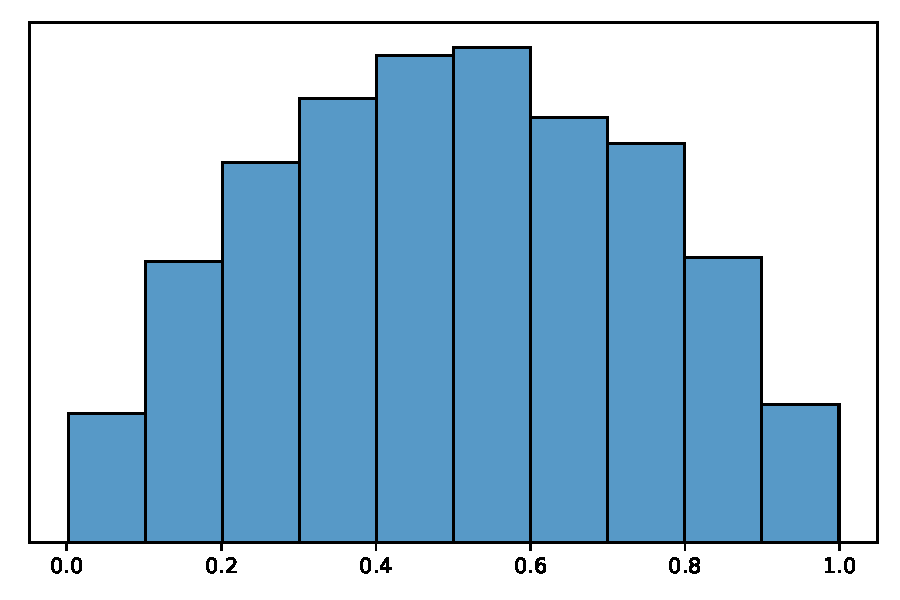
\includegraphics[width=0.3\textwidth]{plots/pit/overdispersed.pdf} \label{fig:pit-overdispersed} }}
    \subfloat[\centering Neturally dispersed]{{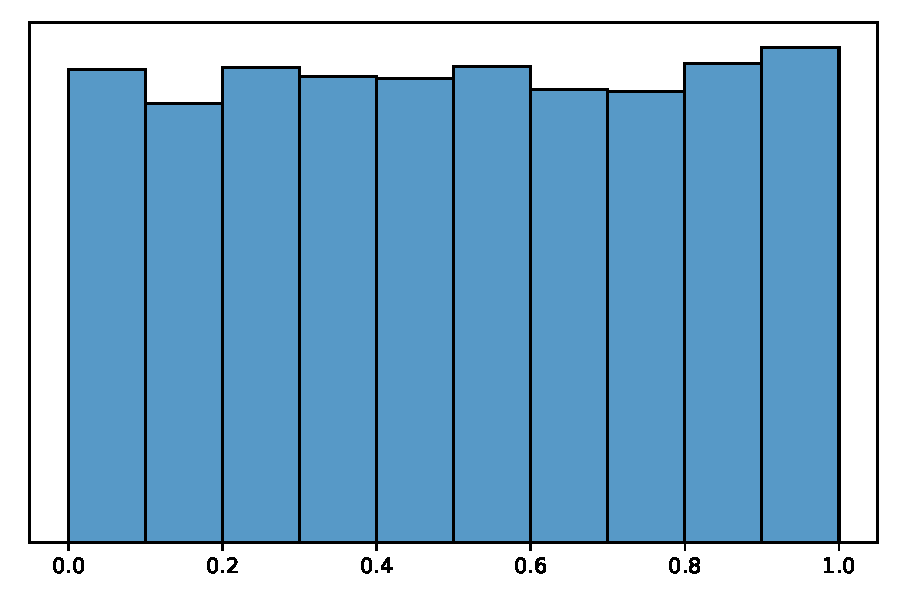
\includegraphics[width=0.3\textwidth]{plots/pit/neutrally_dispersed.pdf} \label{fig:pit-neutrally-dispersed} }}
    \subfloat[\centering Underdispersed]{{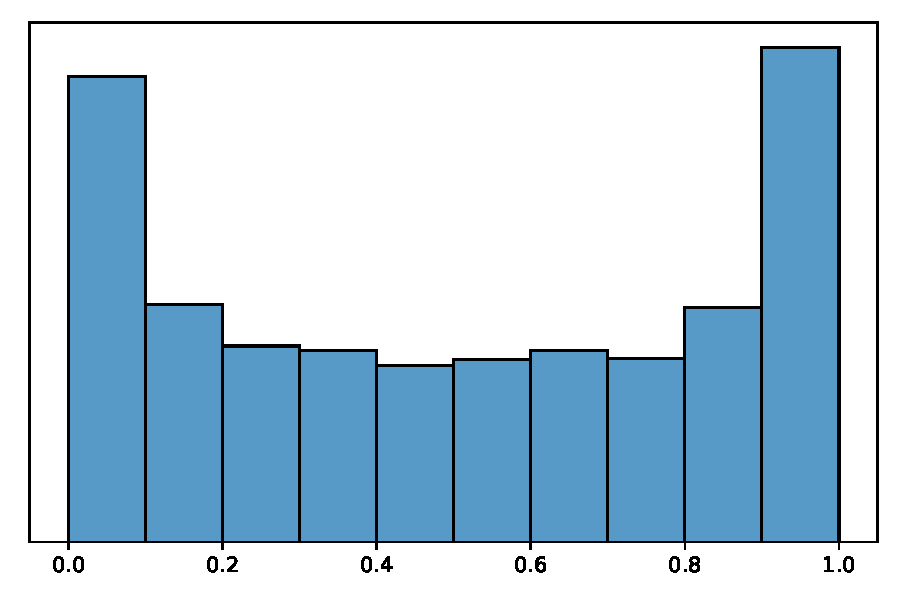
\includegraphics[width=0.3\textwidth]{plots/pit/underdispersed.pdf} \label{fig:pit-underdispersed} }}
    \caption[Dispersion types for PITs]{Dispersion types for PITs. The PIT of an overdispersed forecast is formed like a \(\cap\) (Figure \ref{fig:pit-overdispersed}). 
    Figure \ref{fig:pit-neutrally-dispersed} is probabilistically calibrated, i.e. \(Z_F \sim U(0,1)\), and therefore neutrally dispersed. 
    An underdispersed forecast has a PIT that looks like a \(\cup\) (Figure \ref{fig:pit-underdispersed}).}%
    \label{fig:dispersion}%
\end{figure}

\begin{figure}[h]%
    \centering
    \subfloat[\centering Quantile Random Forests]{{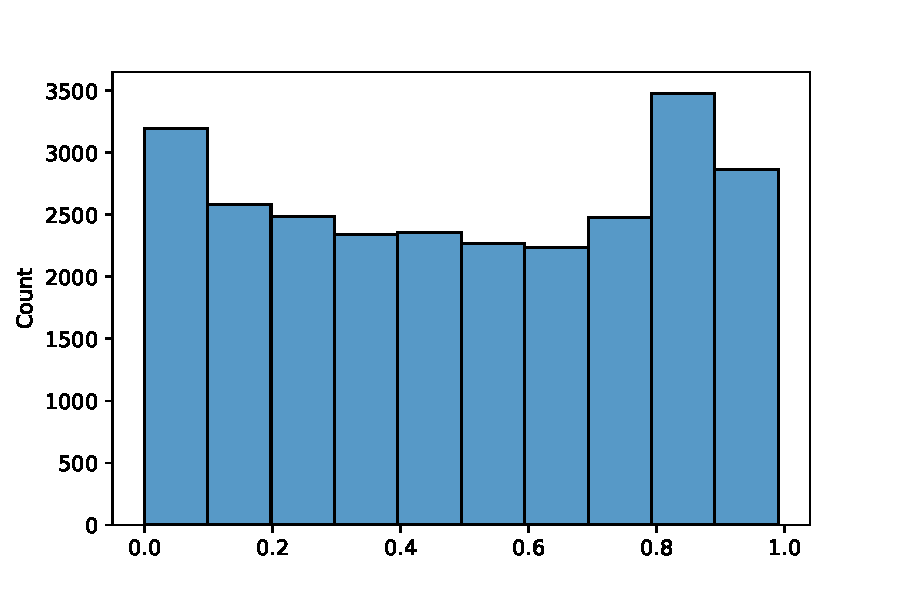
\includegraphics[width=0.45\textwidth]{plots/pit/pit_qrf.pdf} \label{fig:pit-qrf} }}
    \subfloat[\centering Nearest Neighbor Quantile Filters]{{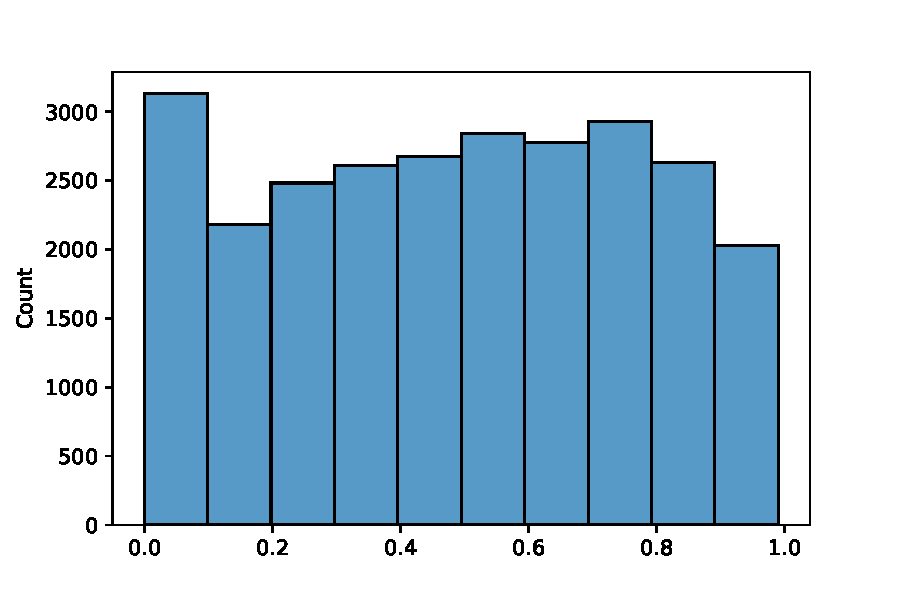
\includegraphics[width=0.45\textwidth]{plots/pit/pit_nnqf.pdf} \label{fig:pit-nnqf} }} \\
    \subfloat[\centering DeepAR]{{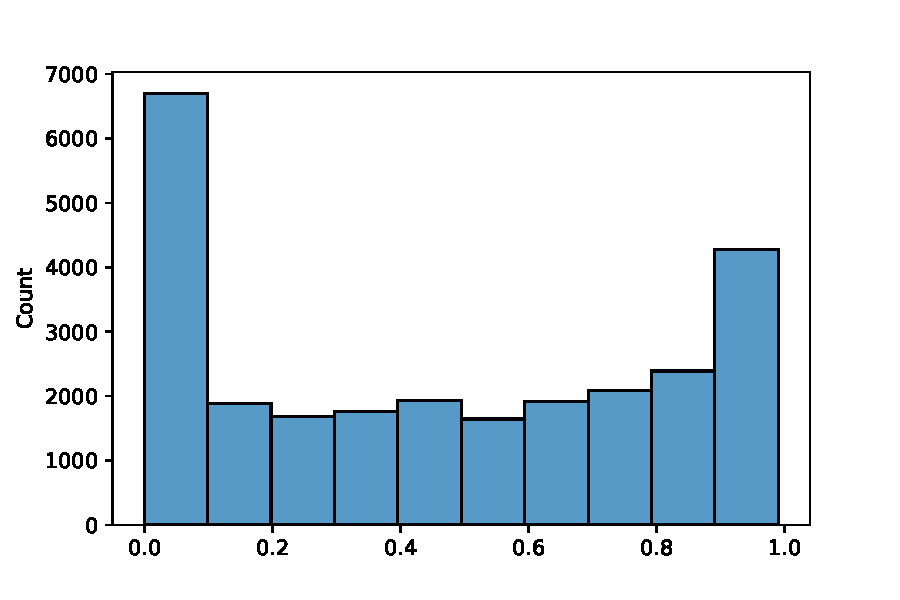
\includegraphics[width=0.45\textwidth]{plots/pit/pit_deepar.pdf} \label{fig:pit-deepar} }}
    \subfloat[\centering Spline Quantile Functions RNN]{{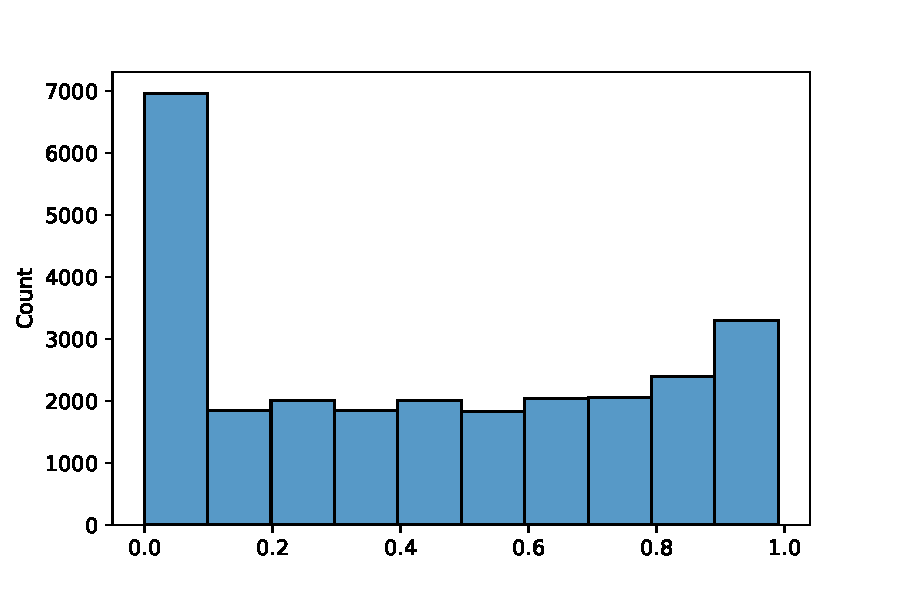
\includegraphics[width=0.45\textwidth]{plots/pit/pit_sqf-rnn.pdf} \label{fig:pit-sqf-rnn} }}
    \caption[PIT histograms]{Probability integral transform of each model. 
    If the distribution of the PIT looks like \(U(0,1)\), it's probabilistically calibrated.}%
    \label{fig:pit}%
\end{figure}

Because the models act differently at each hour, it makes sense 
to look at the PIT histograms for each hour separately. 
The PIT histograms broken down into each hour are shown in Figure \ref{fig:pit-qrf-by-hour}, Figure \ref{fig:pit-nnqf-by-hour}, 
Figure \ref{fig:pit-deepar-by-hour} and Figure \ref{fig:pit-sqf-rnn-by-hour} 
while Figure \ref{fig:pit} shows the PIT histograms averaged over each hour.

One can observe that the PIT histogram of QRF (\ref{fig:pit-qrf}) and NNQF (\ref{fig:pit-nnqf}) are approximately 
\(U(0,1)\)-distributed but the forecasts during the night are overdispersed in the QRF case and 
skewed in the NNQF model.
The DeepAR and SQF-RNN model perform similarly: they are both skewed with a high density at \(0\). 
This means that the actual output lies often in the lower quantiles of the prediction. 